\documentclass[11pt]{article}

\usepackage[T1]{fontenc}
\usepackage{mathptmx}
\usepackage{graphicx}

\topmargin 0.0in
\setlength{\textwidth} {420pt}
\setlength{\textheight} {620pt} 
\setlength{\oddsidemargin} {20pt}
\setlength{\marginparwidth} {72in}

\usepackage{fancyhdr} 
\usepackage{url}

% set it so that subsubsections have numbers and they
% are displayed in the TOC (maybe hard to read, might want to disable)

\setcounter{secnumdepth}{3}
\setcounter{tocdepth}{3}

% define widow protection

\def\widow#1{\vskip #1\vbadness10000\penalty-200\vskip-#1}

\clubpenalty=10000  % Don't allow orphans
\widowpenalty=10000 % Don't allow widows

% this should give me the ability to use some math symbols that 
% were available by default in standard latex (i.e. \Box)

\usepackage{latexsym}

% define a little section heading that doesn't go with any number

\def\littlesection#1{
\widow{2cm}
\vskip 0.5cm
\noindent{\bf #1}
\vskip 0.0001cm 
}

\pagestyle{fancyplain}

\newcommand{\tstamp}{\today}   
\renewcommand{\sectionmark}[1]{\markright{#1}}
\lhead[\Section \thesection]            {\fancyplain{}{\rightmark}}
\chead[\fancyplain{}{}]                 {\fancyplain{}{}}
\rhead[\fancyplain{}{\rightmark}]       {\fancyplain{}{\thepage}}
\cfoot[\fancyplain{\thepage}{}]         {\fancyplain{\thepage}{}}

\newlength{\myVSpace}% the height of the box
\setlength{\myVSpace}{1ex}% the default, 
\newcommand\xstrut{\raisebox{-.5\myVSpace}% symmetric behaviour, 
  {\rule{0pt}{\myVSpace}}%
}

% leave things with no spacing extra spacing in the final version of the paper
\renewcommand{\baselinestretch}{1.0}    % must go before the begin of doc

% suppress the use of indentation for a paragraph

\setlength{\parindent}{0.0in}
\setlength{\parskip}{0.1in}
\setlength{\headheight}{15pt}

\begin{document}

%% \begin{abstract}

%%   Try

%% \end{abstract}

% handle widows appropriately
\def\widow#1{\vskip #1\vbadness10000\penalty-200\vskip-#1}

% build the title section

\makeatletter

\def\maketitle{%
  %\null
  \thispagestyle{empty}%
  %\vfill
  \begin{center}%\leavevmode
    %\normalfont
    {\Huge \@title\par}%
    %\hrulefill\par
    {\normalsize \@author\par}%
    \vskip .4in
%    {\Large \@date\par}%
  \end{center}%
  %\vfill
  %\null
  %\cleardoublepage

  }

\makeatother

\vspace*{-1.1in}
\title{Integration of Real-Time Collaborative Coding with Git for Productivity Gains}

% build the author section
\author{Braden D. Licastro\\
Department of Computer Science\\
Allegheny College \\
{\tt licastb@allegheny.edu}  \\
\url{http://www.fullforceapps.com/} \\ 
\vspace*{.1in} \today \\ \vspace*{.1in}
{\bf Abstract} \\ This paper describes a method of coding to be researched that has the potential to greatly improve efficiency of program development. By combining the effectiveness and flexibility of collaborative coding with a version control system it may be possible to reduce time wasted during the software development cycle and shorten turn around times.}

% use the default title stuff
\maketitle

\vspace*{-.4in}
\section{Introduction}
\label{sec:introduction}
\vspace*{-.1in}

Software development is full of pitfalls that take an innumerable amount of time every year to overcome, especially when working with a group of developers. One major stumbling point every seasoned programmer will experience arises when using a revision control system. When projects are branched for feature work and merged at a later time collisions, otherwise known as conflicts will more than likely occur. The current method of resolving these conflicts is arduous at best, and can even lead to a code freeze until a solution is found. By integrating a version control system with a method of collaborative real-time coding it should be possible to greatly reduce, or even eliminate the chance of conflicts when a project is merged back to the master branch without losing the benefits of a source manages project.

Current implementations of revision control systems are designed to be as intuitive and straightforward as possible, but for the most part remain weak in their handling of errors. Frequent problems arise when two branches of a project must be merged back into one and the code on one conflicts with code in the other. As of the writing of this paper, there is no standardized method of handling these situations. Many times it is required that the developer go back and manually edit the code thus resolving any conflicts. In some instances this is a trivial task, but others it is tedious and time consuming. With real-time collaboration it is possible to have many developers actively working on the same code-base without the necessity of a code merge that may or may not work out of the box. This setup would allow all contributors to see the code as it currently stands on other computers and work together to create code that is conflict free on the fly. This gain in efficiency could add up to be quite considerable, and different implementations may produce significantly beneficial results.

\vspace*{-.1in}
\section{Related Work}
\label{sec:relatedwork}
\vspace*{-.1in}

The topic of collaborative coding is a rather new research topic. Much of the current research resolves around the implementation of an effective environment. One research paper describes a web-based Java development environment that supports collaboration between programmers names Collabode.\cite{Goldman:2011:RCC:2047196.2047215} The system analyzed is web based and has no code management integrated. The implementation I have proposed would be non web based in implementation, and it would have integrated revision control. This paper also talks about the advantages and shortcomings of such technologies, while the proposed research would determine the amount of time that can be saved through a series of surveys. Similar to this paper, the same authors published another article that discusses possible workload reductions by using the Collabode system to outsource small amounts of coding. \cite{Goldman:2011:CCC:1984642.1984658} 

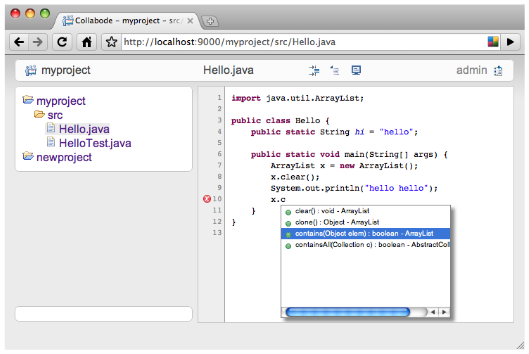
\includegraphics[scale=.7]{collabode}

This research paper describes using the system shown above and gives information relating to how error prone the system is but does not specifically outline any gains or losses from using this versus a traditional approach to coding. In the second paper, the Collabode implementation is tested using the same parameters that gathered the error data in the previous paper, but elaborates slightly. The addition of test suites allows a test for the correctness of the code, not just ensuring it compiles. \cite{Goldman:2011:RCC:2047196.2047215} Several other papers discuss similar concepts of collaborative editing, but only discuss implementation techniques such as using collaborative editors in a classroom session to promote pair programming and learning cooperatively. \cite{Hickey:2005:ECP:1040196.1040215} Another paper exists to explain the process of integrating a collaborative code editing feature into the eclipse platform. \cite{Waldmann:2010:IGW:1867651.1867671}

\vspace*{-.2in}
\section{Method of Approach}
\label{sec:method}
\vspace*{-.1in}

The proposed research will look at existing data from research articles such as the paper outlining the Collabode systems and also utilize a survey and timing system to gauge real world use in an educational facility. The given data as seen below shows the statistics from an existing test. In this case there were members of the research team utilizing the software and their performance while collaborating was recorded.

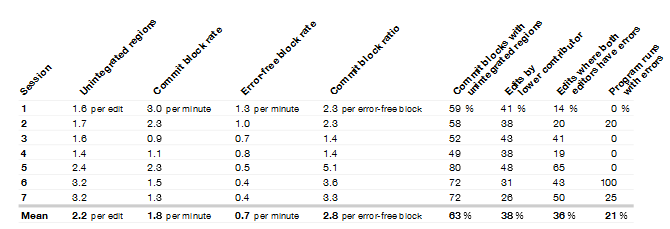
\includegraphics[scale=.7]{stats}

Due to the small amount of research in this area it will be relatively simple to compile all of the current data into a workable set that will represent the basis for research. By using this laboratory style test data, I will compare it to real world results gathered through surveys and data gathered from undergraduate level computer science courses in order to find what environments lend themselves to better performance.

\vspace*{-.2in}
\section{Evaluation Strategy}
\label{sec:evaluate}
\vspace*{-.1in}

In order to gather data that can be evaluated there will be set guidelines that will be followed in order to ensure consistency. When collecting preexisting data, it must be gathered in a lab setting as the data for the Collabode software research project was. In addition, when testing the collaborative coding environment in an educational facility, the data will only be collected for upperclassmen whom have had ample experience using various environments and languages. In addition, it is to be tested using an environment that supports full user collaboration including inline chat, editing that is real-time and visible to both parties, similar to the setup in the figure below.

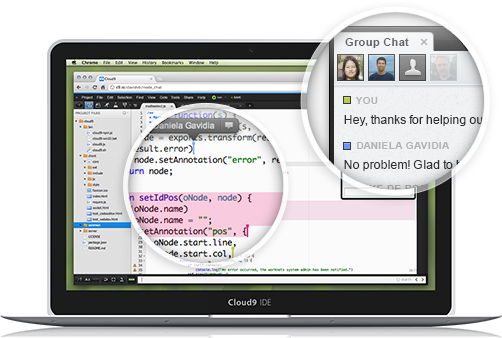
\includegraphics[scale=.5]{collab-feature}

\vspace*{-.1in}
\section{Research Schedule}
\label{sec:schedule}
\vspace*{-.1in}

To begin the project several topics must be addressed, namely the precise setup, method of benchmarking and data collection, and the data evaluation itself. Within the first two to four weeks of beginning the project I will research availability of collaborative coding environments and which one is best suited for this research. In addition accompanying programs will be coded that record various metrics in the collaborative environment and emacs. The data to be collected will be active coding time, error frequency, for example syntax, compile time, and run time errors. It will also record the length of the code and how much input each user has provided and the overall code length for the given project.

Phase 1 - 3 weeks: To begin the research process I will choose a platform in which I am going to implement an existing collaborative code environment, choosing one with the least learning curve.

Phase 2 - 1 week: Set up coding environment on computers and test to make sure everything is working properly. If not work out any bugs.

Phase 3 - 1 month: Allow computer science classes to use coding environment in group projects. After using the environment for this duration of time they will be familiar with its workings and I will have had time to work out any unexpected problems.

Phase 4 - 4 weeks: Instruct one half of computer science class to work in groups in a traditional manner, while the other uses the new environment. During this process they will report any problems or difficult situations they had during the process. In addition, the program will collect data such as various errors, for example runtime, compile time, et cetera. The program will also gauge the amount of time spent actively coding during the class session vs the amount of time spent collaborating off screen.

Phase 5 - 3-6 weeks: Gather data from the computers and the reports each student filled out with problems they encountered. From this data I will be able to determine patterns and various metrics such as inefficient time spent collaborating off screen when working cooperatively and average code error percentages. Record all data in one place for easy review and begin organizing it in an intuitive and manner using graphs and various other visual aides.

Phase 6 - remaining time: Complete the evaluation of results and organize thoughts in a way that is presentable to readers unfamiliar with the research performed. Complete research, determine flaws in method, and report new ways to expand or improve upon findings for future projects.

\vspace*{-.1in}
\section{Conclusion}
\label{sec:conclusion}
\vspace*{-.1in}

Using collaborative code environments may dramatically improve productivity and output of programmers. Traditionally, programming would be done on individual machines by groups of people and must be merged into a parent project at a later point in time. This creates a large inefficiency as collisions, conflicts, and incompatible code take a vast amount of time to resolve that could be used to further develop or test a piece of software. By using collaborative environments it is possible, in theory, to eliminate these inefficiencies as the code is never branched. In addition, while multiple programmers work within the same document it is possible to assist others without the need to collaborate off screen and come back to solve a problem. Having all of the code at hand allows all programmers a better understanding of what the other is doing, and creates a better environment for easy communication.

By testing this hypothesis, it could be possible to change the way coding is completed if the results are favorable. It is possible that other inefficiencies can be discovered and addressed that were unexpected or otherwise little known. The direct impact on the field of computer science could be great, with new research in environment optimization tools, code efficiency gains through collaboration, or possibly even a way to avoid conflicts, therefore reducing wasted time due to errors.

As a future topic of study, researching the possibility of a combined source management system with cooperative, live code modification could prove very effective. By doing this, the benefit of revision control could be exploited while addressing its weaknesses.  

\bibliographystyle{plain}
\bibliography{senior_thesis_proposal}

\end{document}

